\documentclass[border=4pt]{standalone}
\usepackage{tikz}
\usepackage{pgfplots}
\pgfplotsset{compat=1.18}
\usetikzlibrary{shapes.geometric,arrows.meta,positioning,calc,fit,decorations.pathreplacing,backgrounds}
\definecolor{boxblue}{RGB}{225,238,252}
\definecolor{boxgreen}{RGB}{225,247,231}
\definecolor{boxorange}{RGB}{253,236,216}
\definecolor{boxgray}{RGB}{237,237,237}
\definecolor{boxred}{RGB}{253,226,226}
\begin{document}
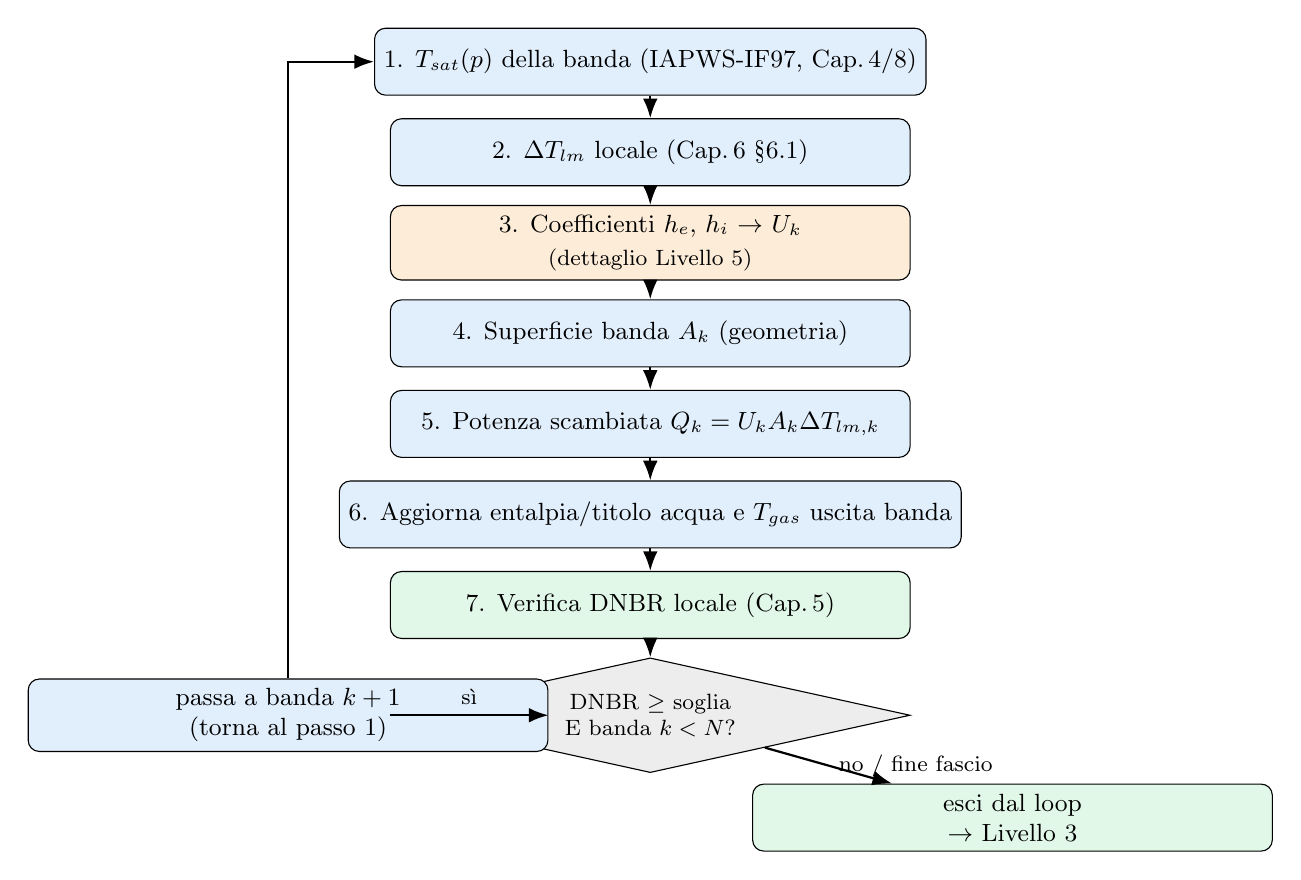
\begin{tikzpicture}[
  box/.style={draw, rectangle, rounded corners, minimum height=0.85cm, minimum width=6.6cm, align=center, font=\small},
  dec/.style={draw, diamond, aspect=3, align=center, font=\footnotesize, inner sep=2pt, minimum width=6.6cm},
  arr/.style={-{Latex[length=2.5mm]}, thick}
]
\node[box, fill=boxblue] (n1) at (0,0) {1. $T_{sat}(p)$ della banda (IAPWS-IF97, Cap.\,4/8)};
\node[box, fill=boxblue] (n2) at (0,-1.15) {2. $\Delta T_{lm}$ locale (Cap.\,6 \S6.1)};
\node[box, fill=boxorange] (n3) at (0,-2.3) {3. Coefficienti $h_e$, $h_i$ $\rightarrow$ $U_k$\\[1pt]\footnotesize (dettaglio Livello 5)};
\node[box, fill=boxblue] (n4) at (0,-3.45) {4. Superficie banda $A_k$ (geometria)};
\node[box, fill=boxblue] (n5) at (0,-4.6) {5. Potenza scambiata $Q_k = U_k A_k \Delta T_{lm,k}$};
\node[box, fill=boxblue] (n6) at (0,-5.75) {6. Aggiorna entalpia/titolo acqua e $T_{gas}$ uscita banda};
\node[box, fill=boxgreen] (n7) at (0,-6.9) {7. Verifica DNBR locale (Cap.\,5)};
\node[dec, fill=boxgray] (dec) at (0,-8.3) {DNBR $\ge$ soglia\\ E banda $k<N$?};
\node[box, fill=boxblue] (nextband) at (-4.6,-8.3) {passa a banda $k+1$\\ (torna al passo 1)};
\node[box, fill=boxgreen] (endloop) at (4.6,-9.6) {esci dal loop\\ $\rightarrow$ Livello 3};

\draw[arr] (n1) -- (n2);
\draw[arr] (n2) -- (n3);
\draw[arr] (n3) -- (n4);
\draw[arr] (n4) -- (n5);
\draw[arr] (n5) -- (n6);
\draw[arr] (n6) -- (n7);
\draw[arr] (n7) -- (dec);
\draw[arr] (dec) -- node[above,font=\footnotesize]{sì} (nextband);
\draw[arr] (nextband) |- (n1);
\draw[arr] (dec) -- node[right,font=\footnotesize]{no / fine fascio} (endloop);
\end{tikzpicture}
\end{document}
